\chapter{Delotoki v Orangeu}
\label{ch:workflows}

\newthought{Delotoki v Orangeu} so sestavljeni iz komponent, ki berejo, procesirajo in prikazujejo podatke. Te komponente imenujemo gradniki. Na desni je prazen prostor, t.i. platno. Nanj polagamo gradnike. Gradniki v Orangeu komunicirajo preko komunikacijskih kanalov. Izhod iz enega gradnika je uporabljen kot vhod za drug gradnik.

\begin{figure*}[h]
  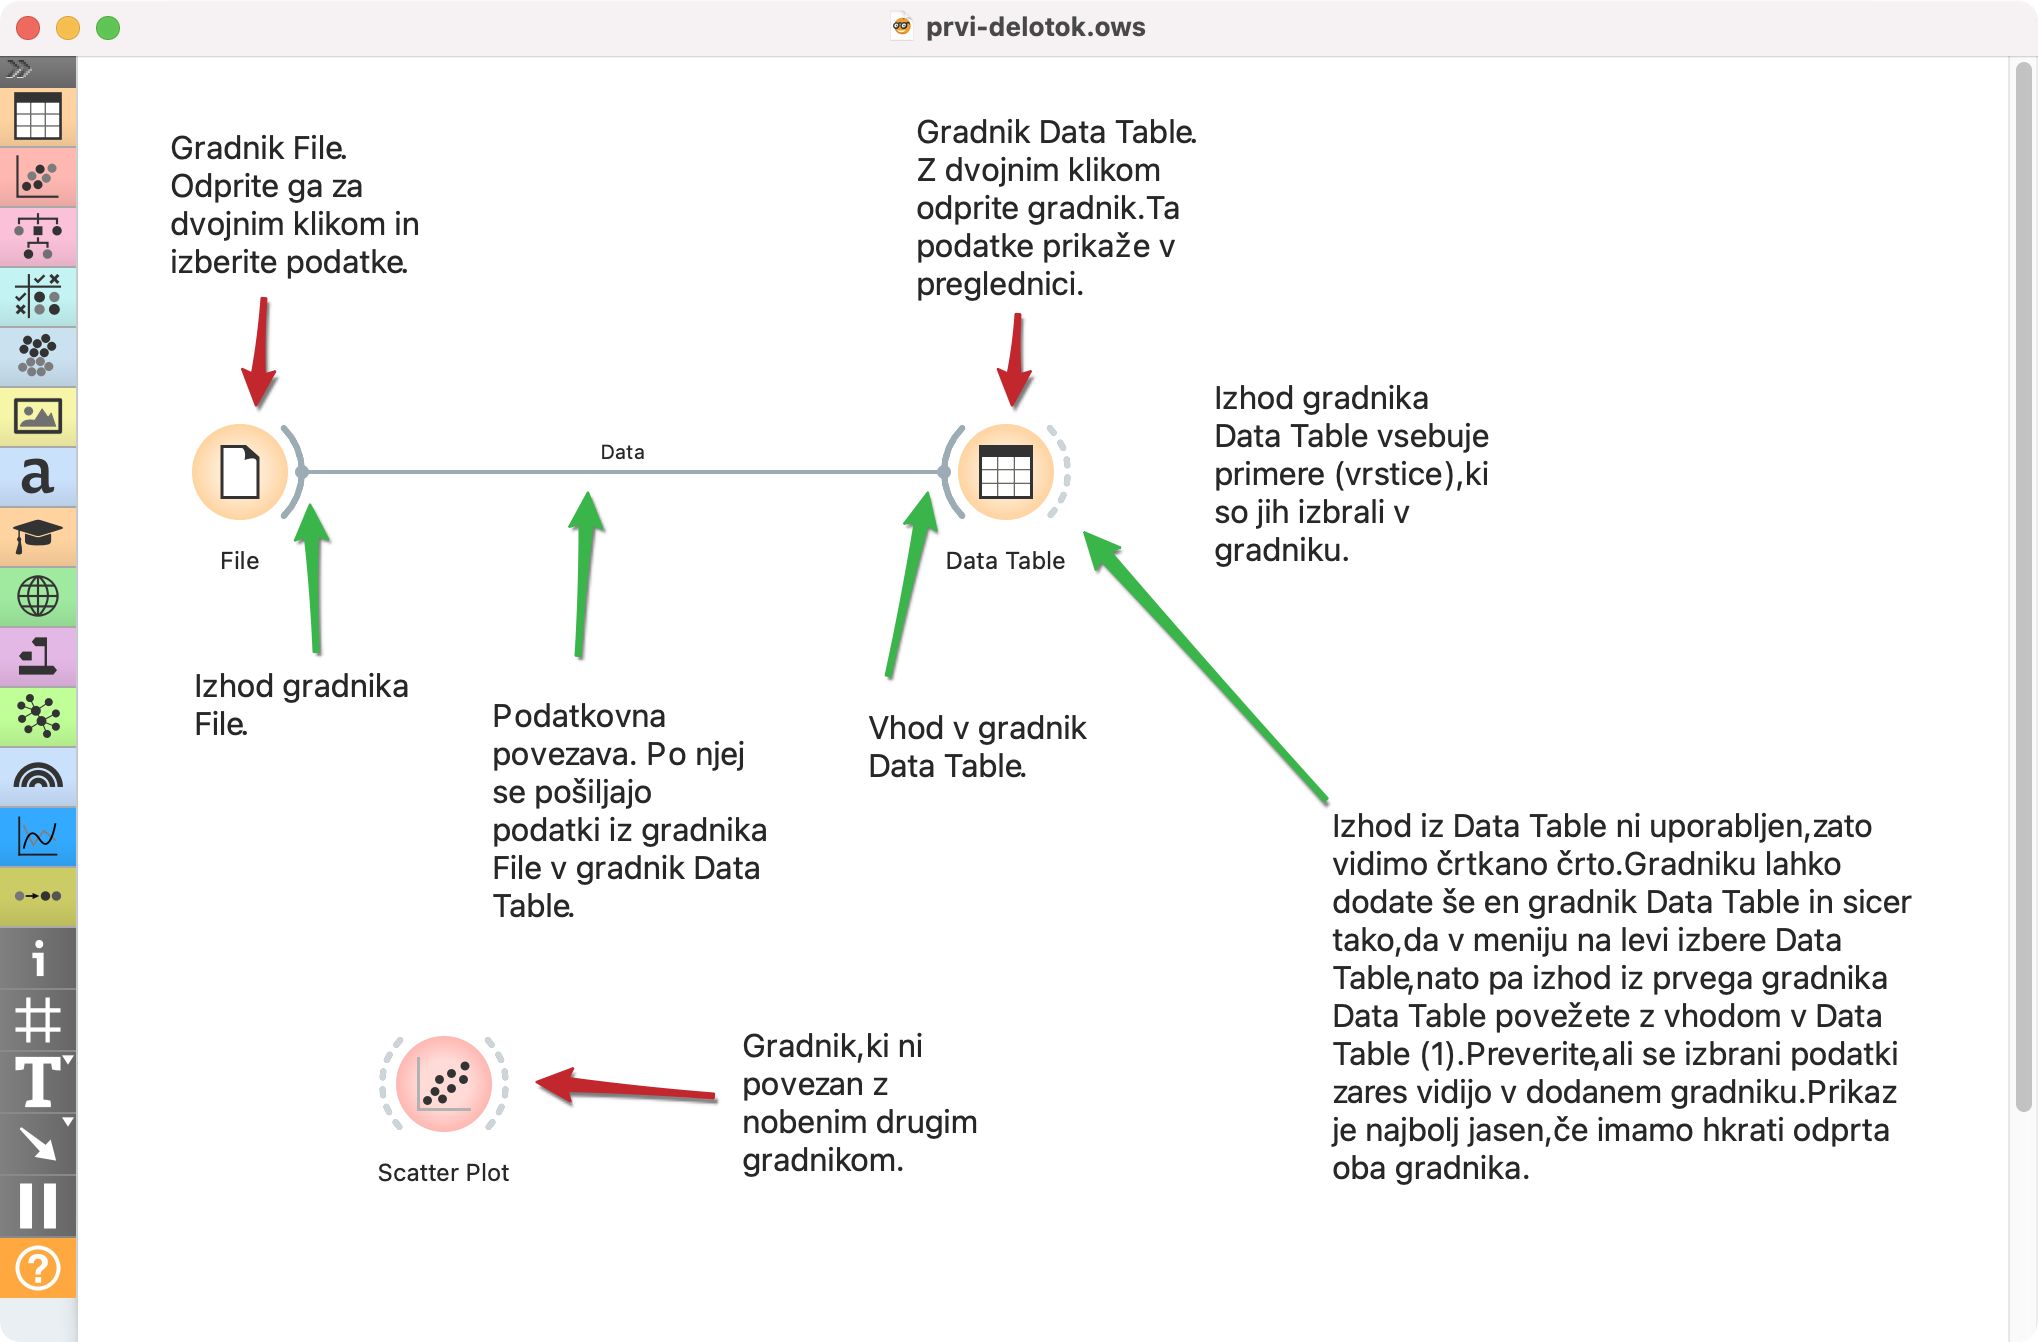
\includegraphics[width=\linewidth]{prvi-delotok.png}%
  \caption{Slika zgoraj kaže preprost delotok z dvema povezanima gradnikoma in enim gradnikom brez povezav. Izhodi gradnika so na desni strani, vhodi pa na levi.}
  \label{fig:workflow-fig1}
\end{figure*}

Delotoke sestavljamo tako, da polagamo gradnike na platno in jih povezujemo. Povezavo ustvarimo tako, da potegnemo črto od izhodnega v vhodni gradnik. Izhodi gradnika so na desni, vhodi pa na levi strani. V zgornjem delotoku gradnik \widget{File} pošilja podatke v gradnik \widget{Data Table}.

\newpage

Pričnite z gradnjo delotoka, ki vsebuje gradnik \widget{File}, dva gradnika \widget{Scatter Plot} in gradnika \widget{Data Table}:

\begin{figure}[h]
  \centering
  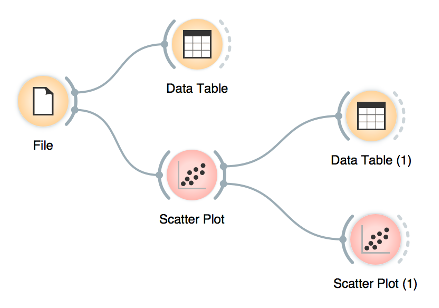
\includegraphics[width=0.9\linewidth]{workflow-fig2.png}%
  \caption{Delotok z gradnikom File bere podatke iz računalnika in jih pošlje v gradnika Data Table in Scatter Plot. Data Table prikaže podatke v preglednici, Scatter Plot pa jih vizualizira. Izbrane točke iz Scatter Plota so poslane v naslednja gradnika, Data Table (1) in Scatter Plot (1).}
  \label{fig:workflow-fig2}
\end{figure}

Gradnik \widget{File} bere podatke z lokalnega diska. Odprite File tako, da dvakrat kliknete na ikono. Orange že vsebuje nekaj prednaloženih korpusov. Iz spustnega menija izberite \textit{heart-disease.tab}, podatke o prisotnosti srčno-žilnih bolezni pri pacientih.

\begin{figure}[h]
  \centering
  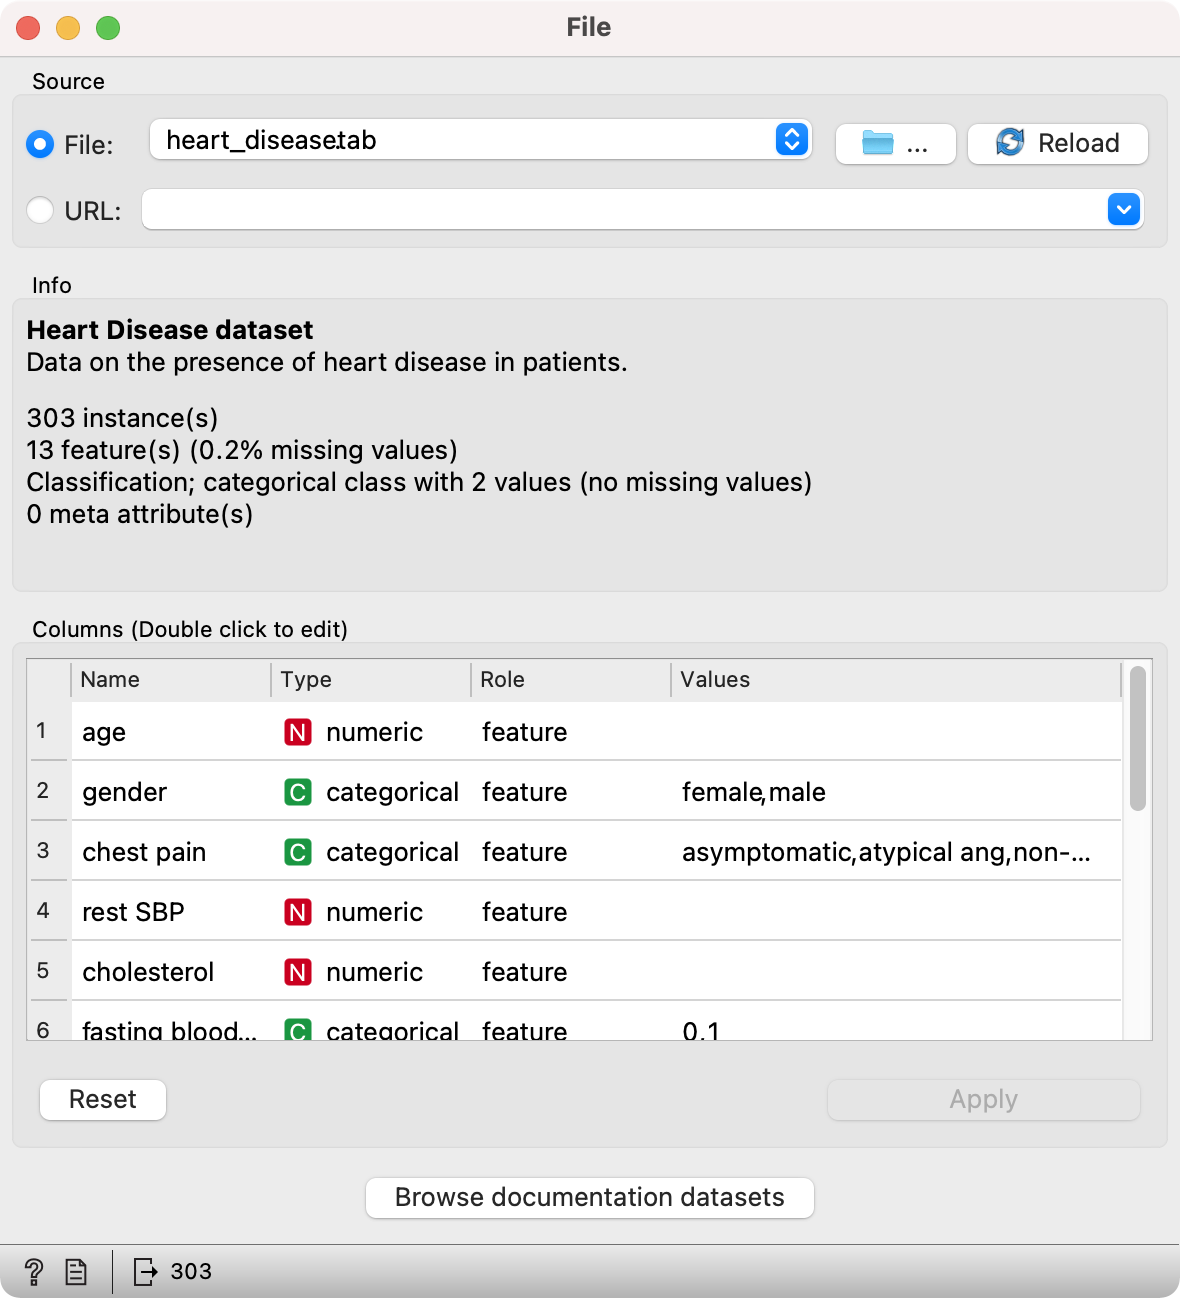
\includegraphics[width=0.8\linewidth]{heart-disease.png}%
  \caption{Orangevi delotoki se pogosto pričnejo z gradnikom File. Podatki o srčno-žilnih boleznih vsebujejo 303 vrstice (paciente) in 14 spremenljivk.  Od 14 stolpcev jih 13 vsebuje podatke o pacientu, en stolpec pa vsebuje informacijo o tem, ali ima pacient srčno bolezen ali ne.}
  \label{fig:heart-disease}
\end{figure}

Ko naložimo podatke, odprimo preostale gradnike. V razsevnem diagramu izberimo nekaj točk in opazujmo, kako se pojavijo v gradniku Data Table (1). Uporabite kombinacijo dveh razsevnih diagramov, kjer drugi diagram prikaže podmnožico, ki ste jo izbrali v prvem.

Povežite izhod gradnika Data Table z gradnikom Scatter Plot (glej spodaj). Odstranite preostala gradnika tako, da ju izberete in pritisnete Delete. Nato izberite vrstico v Data Table in preverite Scatter Plot. Primer, ki ste ga izbrali v preglednici, je sedaj označen v razsevnem diagramu! Uporabite puščice za sprehajanje po vrsticah ali pa s tipko Shift izberite več vrstic hkrati.

\begin{figure}[h]
  \centering
  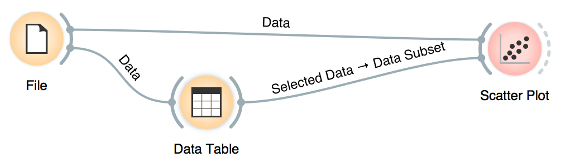
\includegraphics[width=\linewidth]{workflow-fig5.png}
\end{figure}

V zgornjem delotoku ima Scatter Plot dva vhoda, podatke iz gradnika File in izbor iz gradnika Data Table. Kako Orange razlikuje med primarnim virom podatkov in izborom? Prvi povezani signal uporabi kot celotne podatke, drugi signal pa kot podmnožico. Nastavitve lahko spremenite ali preverite tako, da dvakrat kliknete na povezavo med gradnikoma.

\begin{figure}[h]
    \centering
    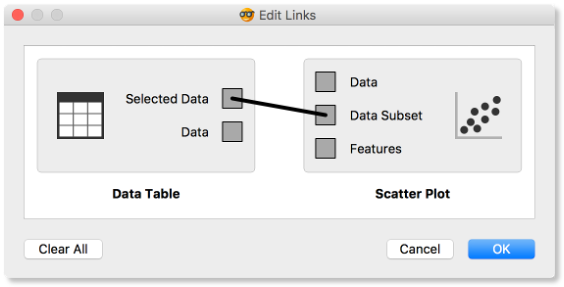
\includegraphics[width=\linewidth]{workflow-fig6.png}
  \end{figure}
  